
We present the PDFs of the inputs of the dynamical simulation and the
output PDFs of the outputs after applying the polarization prior in
addition to the default priors.
%make use of subplots from matplotlib in order to plot all the posteriors
\label{app: results}

%%%%%%%%%%%%% TASK --- 

\clearpage
\begin{figure*}
	\begin{minipage}{180mm}
	\begin{center}
	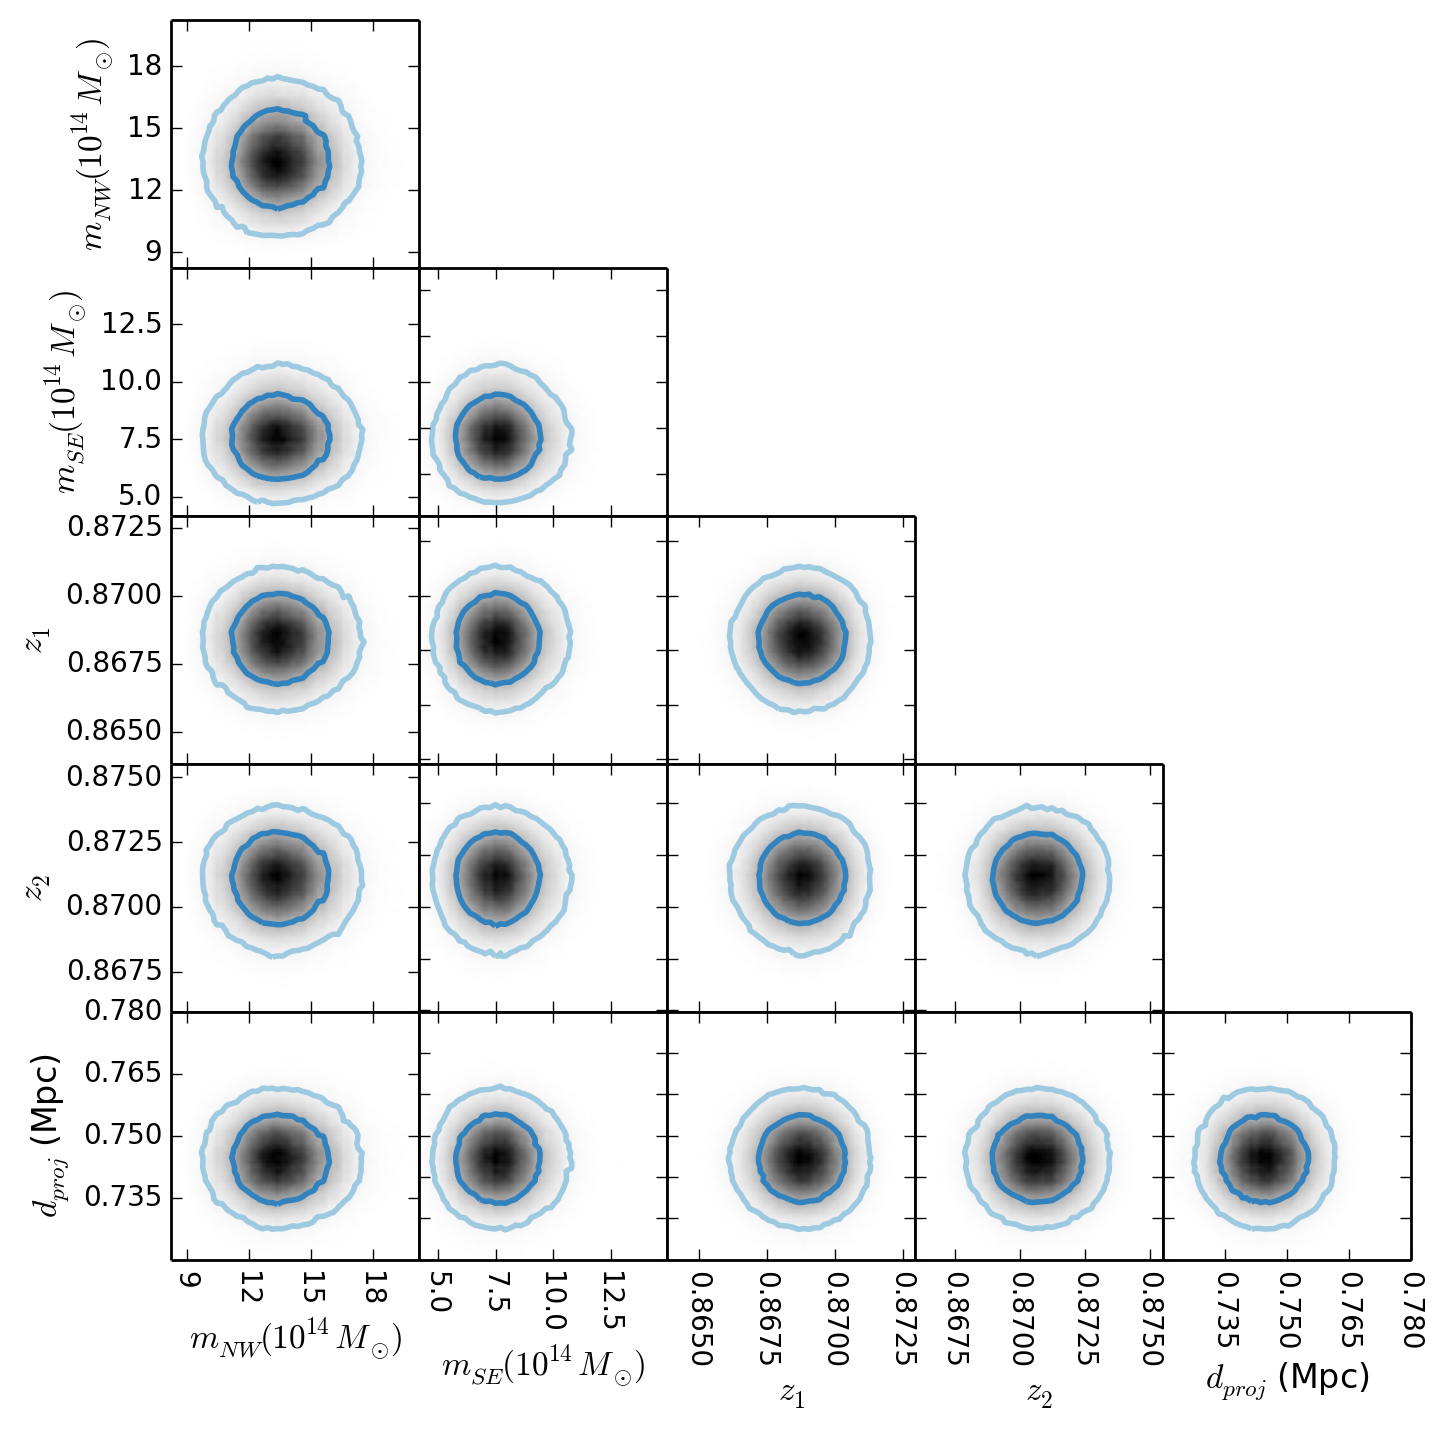
\includegraphics[width=0.65\linewidth]{TwoMnWBSG_inputsVsinput.png}
	\caption{Marginalized PDFs of original inputs and the inputs after
applying polarization prior and default priors. The inner and outer contour
denote the 68\% and 95\% bias-corrected confidence levels respectively.
Circular contours show that priors did not introduce even sampling of
inputs. }
	\end{center}
	\end{minipage}
\end{figure*}

\begin{figure*}
\begin{minipage}{180mm}
	\begin{center}
	%\vspace{200px}
	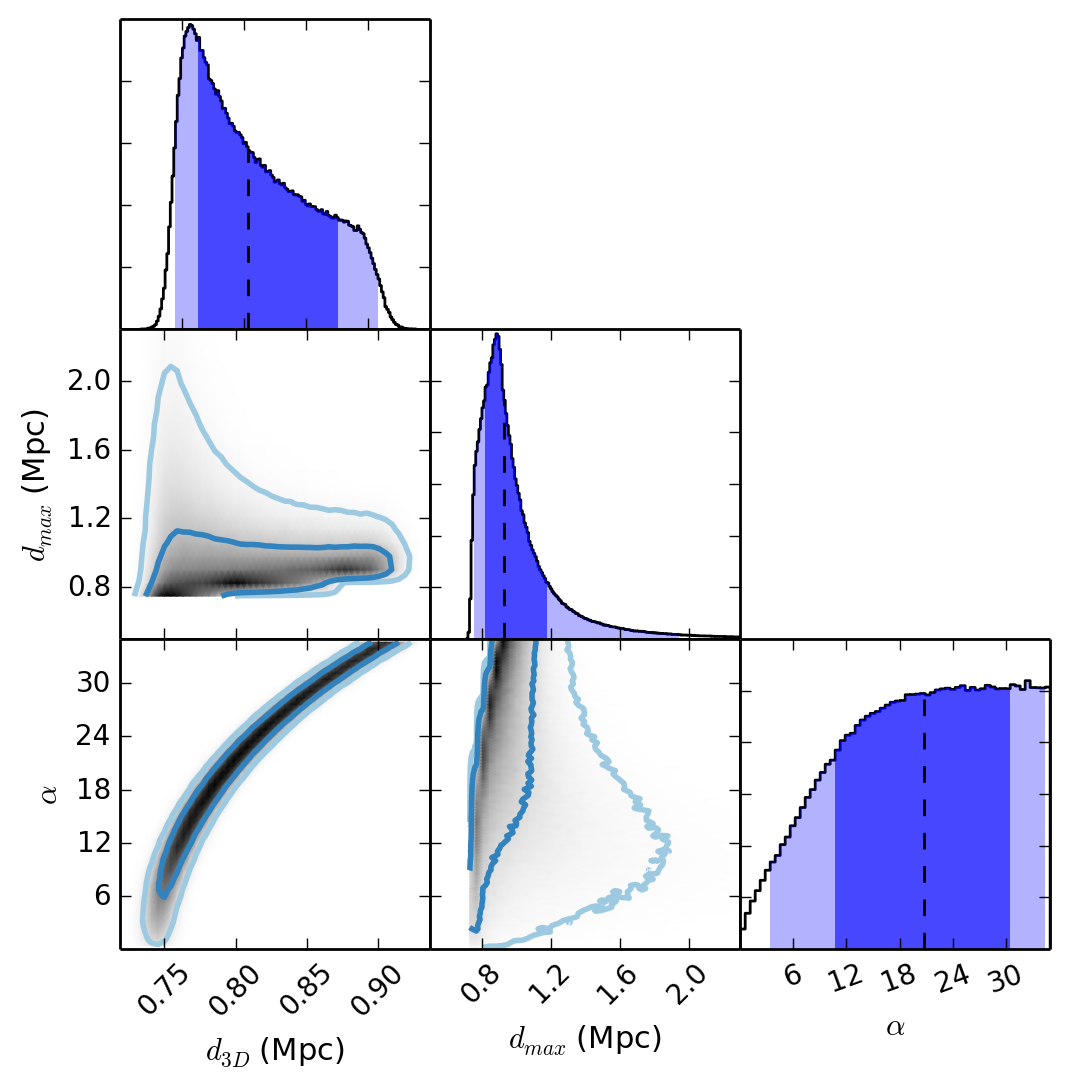
\includegraphics[width=0.5\linewidth]{TwoMnWBSG_tri_geo.png}
	\caption{One-dimensional marginalized PDFs (panels on the diagonal) and
		two-dimensional marginalized PDFs of variables
		denoting characteristic distances and projection angle of the mergers.}
	\end{center}
	\end{minipage}
\end{figure*}

\begin{figure*}
\begin{minipage}{180mm}
	\begin{center}
	%\vspace{200px}
	\includegraphics[width=0.7\linewidth]{TwoMnWBSG_geoVsinputs.png}
	\caption{Marginalized PDFs of characteristic distances and projection
		angle of the merger and the inputs of the simulation.}
	\end{center}
	\end{minipage}
\end{figure*}

\begin{figure*}
\begin{minipage}{180mm}
	\begin{center}
	%\vspace{200px}
	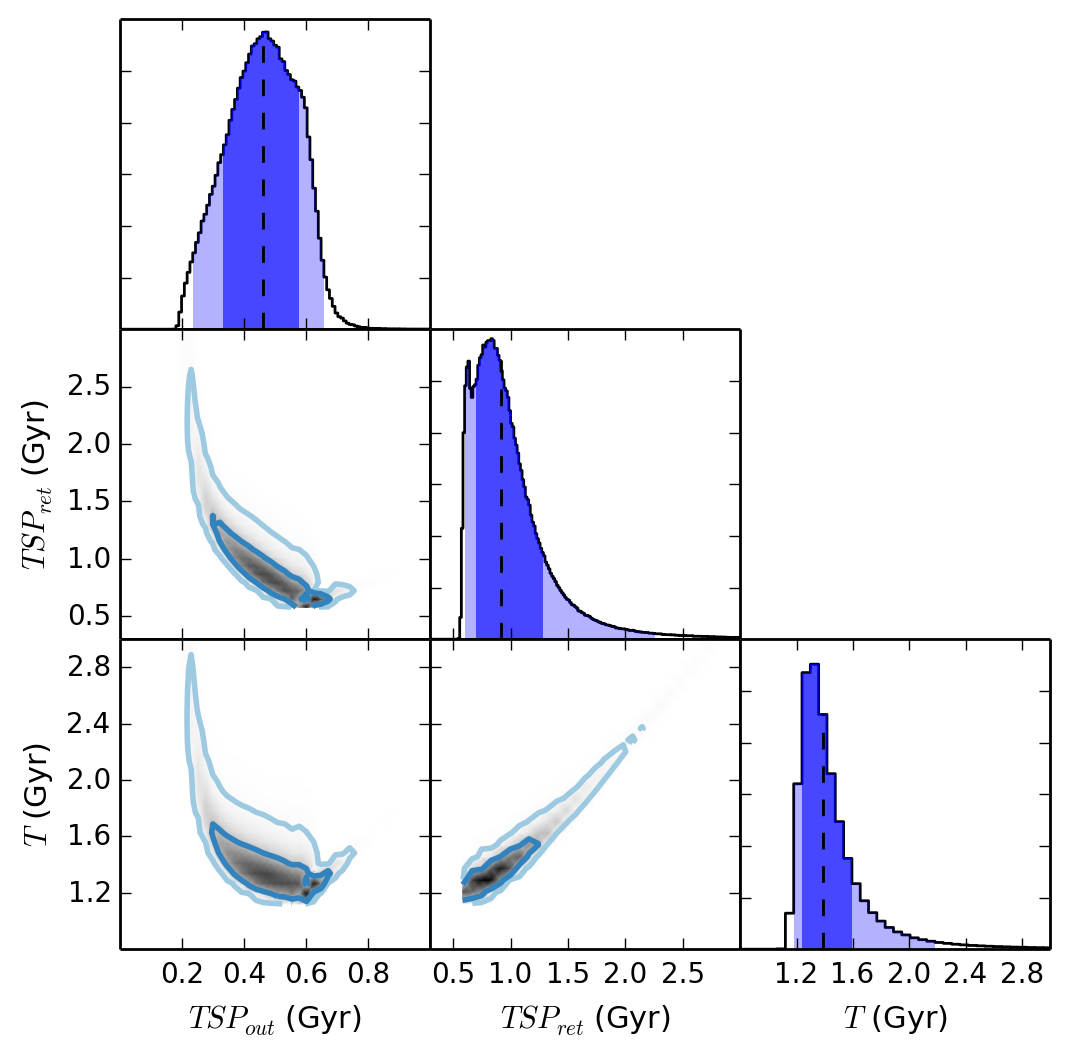
\includegraphics[width=0.5\linewidth]{TwoMnWBSG_tri_time.png}
	\caption{One-dimensional PDFs of characteristic timescales of the simulation
(panels on the diagonal) and the marginalized PDFs of different timescales.}
	\end{center}
\end{minipage}
\end{figure*}

\begin{figure*}
\begin{minipage}{180mm}
	\begin{center}
	%\vspace{200px}
	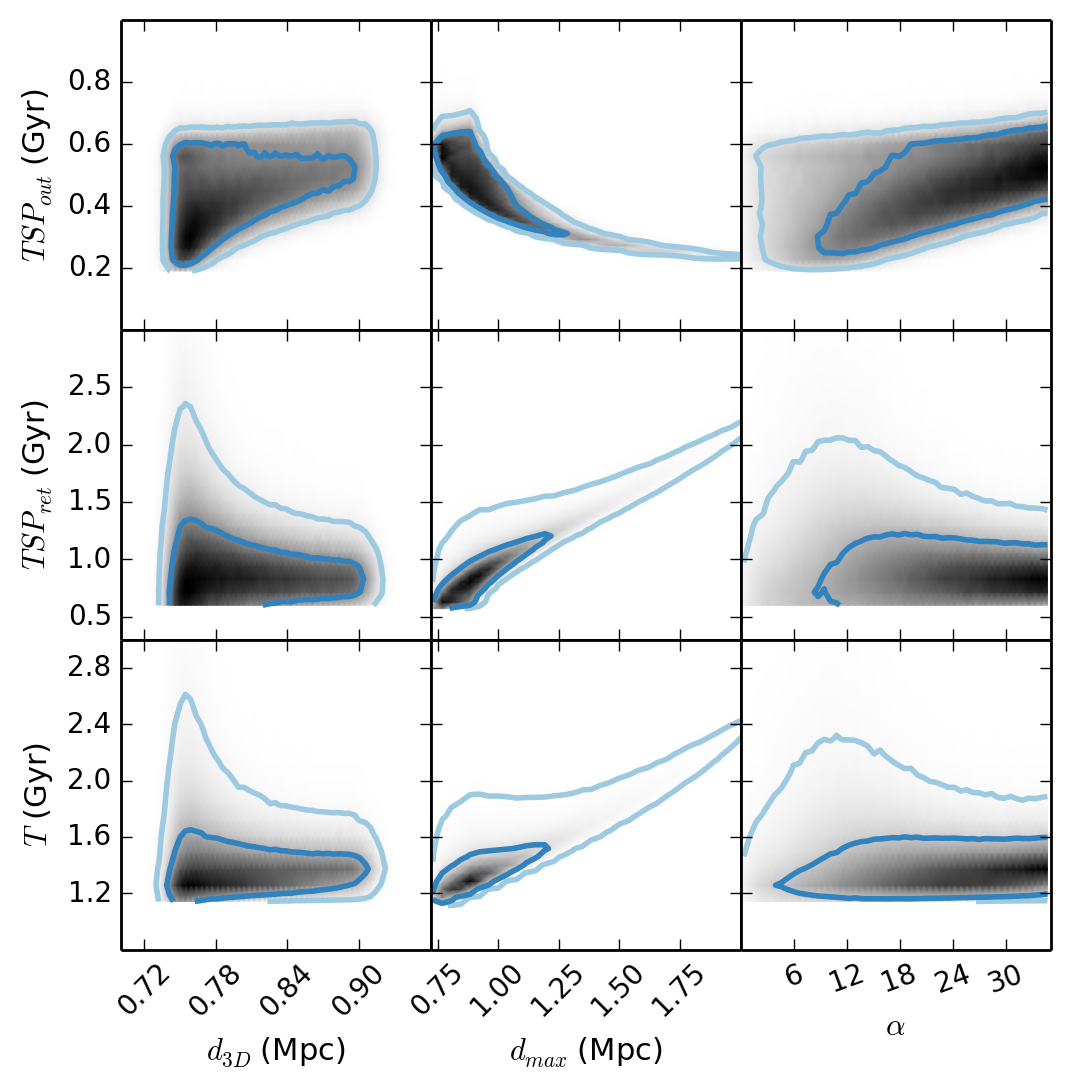
\includegraphics[width=0.5\linewidth]{TwoMnWBSG_timeVsgeo.png}
	\caption{Marginalized PDFs of characteristic timescales of the simulation
and the characteristic distances and the projection angle of the merger. }
	\end{center}
\end{minipage}

\end{figure*}

\begin{figure*}
\begin{minipage}{180mm}
	\begin{center}
	%\vspace{200px}
	\includegraphics[width=0.7\linewidth]{TwoMnWBSG_timeVsinput.png}
	\caption{Marginalized PDFs of characteristic timescales of the simulation
and the inputs.}
	\end{center}
\end{minipage}
\end{figure*}

\begin{figure*}
\begin{minipage}{180mm}
	\begin{center}
	%\vspace{200px}
	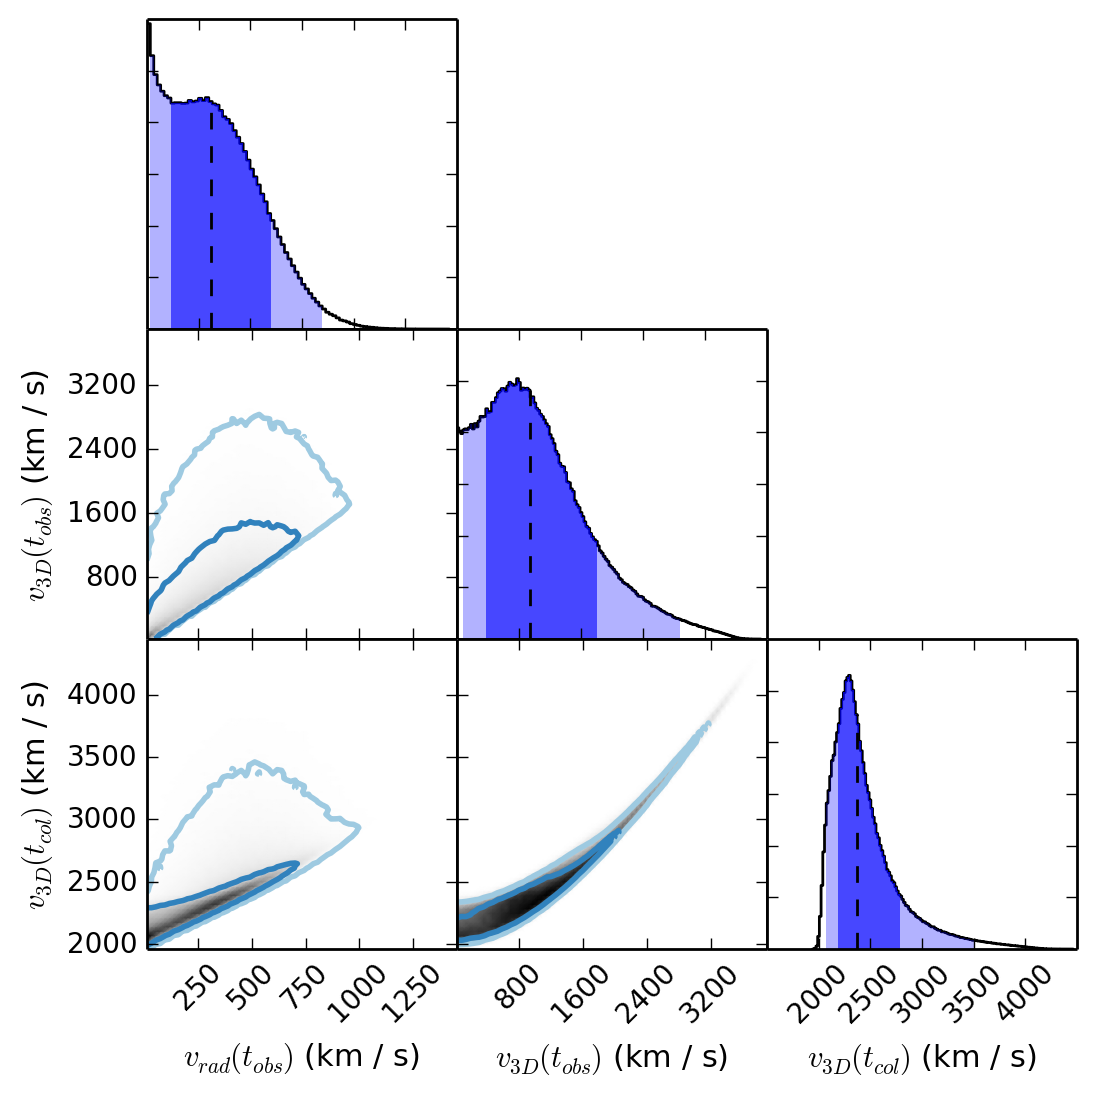
\includegraphics[width=0.5\linewidth]{TwoMnWBSG_tri_vel.png}
	\caption{One-dimensional marginalized PDFs of velocities at
	characteristic times (panels on the diagonal) and marginalized PDFs of
different velocities.}
	\end{center}
\end{minipage}
\end{figure*}

\begin{figure*}
\begin{minipage}{180mm}
	\begin{center}
	%\vspace{200px}
	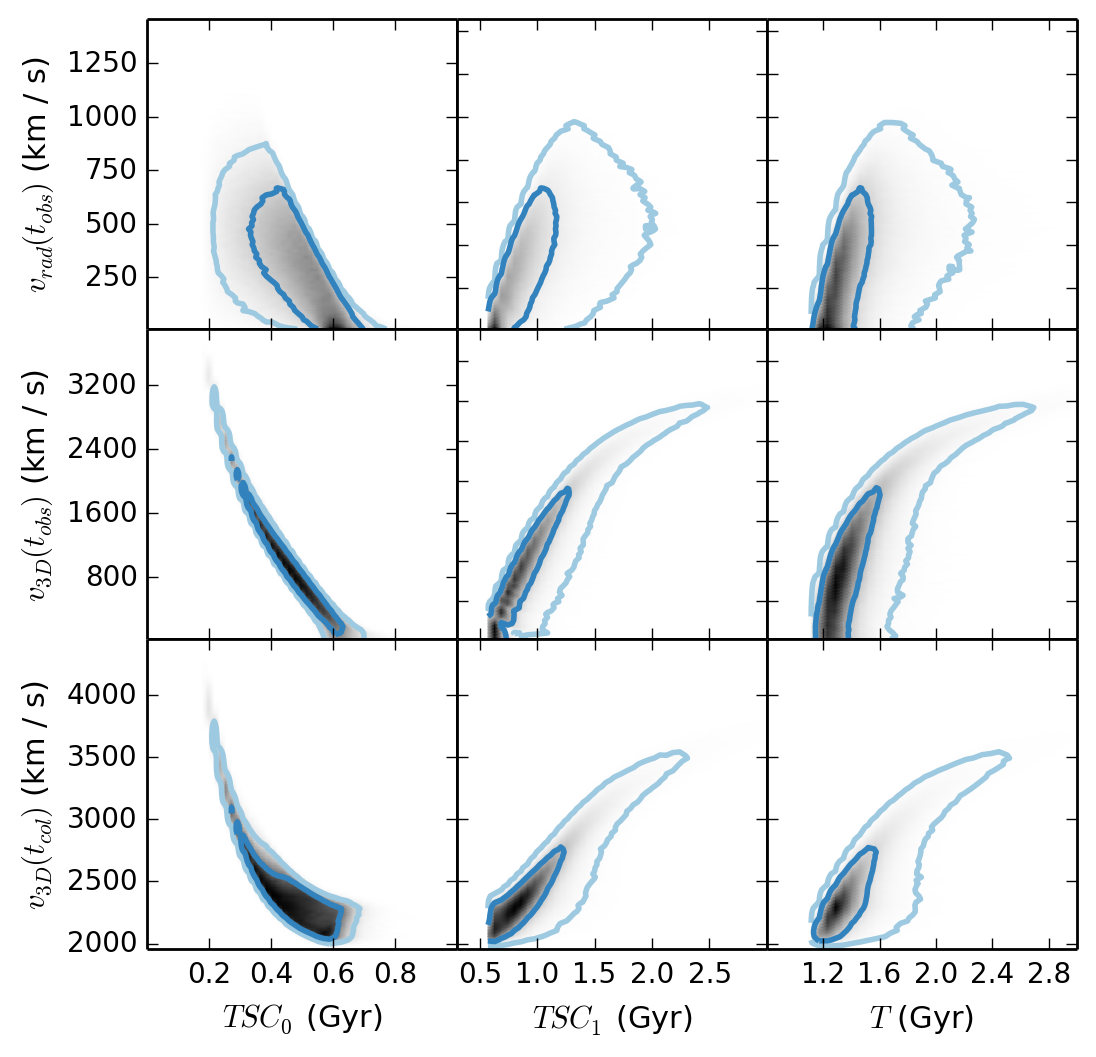
\includegraphics[width=0.5\linewidth]{TwoMnWBSG_velVStime.png}
	\caption{Marginalized PDFs velocities and the characteristic timescales
	of the simulation against the inputs.}
	\end{center}
\end{minipage}
\end{figure*}

\begin{figure*}
\begin{minipage}{180mm}
	\begin{center}
	%\vspace{200px}
	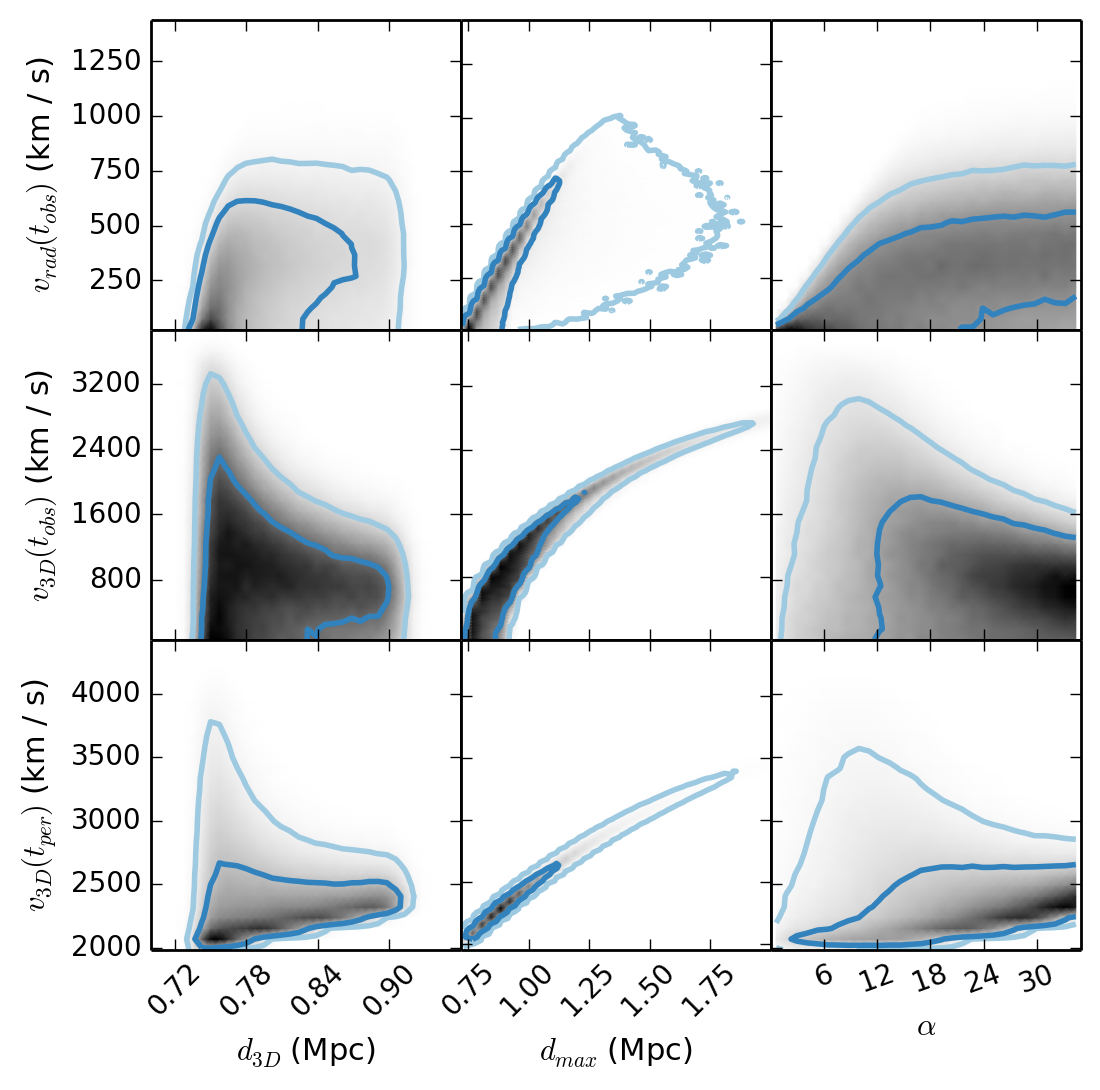
\includegraphics[width=0.5\linewidth]{TwoMnWBSG_velVSgeo.png}
	\caption{Marginalized PDFs of the velocities at characteristic timescales
		and the characteristic distances and the projection angle of the merger. }
	\end{center}
\end{minipage}
\end{figure*}

\begin{figure*}
\begin{minipage}{180mm}
	\begin{center}
	%\vspace{200px}
	\includegraphics[width=0.7\linewidth]{TwoMnWBSG_velVsinputs.png}
	\caption{Marginalized PDFs of relative velocities characteristic
	timescales of the simulation and the inputs.}
	\end{center}
\end{minipage}
\end{figure*}

